\documentclass[border=15pt]{standalone}
\usepackage{tikz}
\tikzset{
  treenode/.style = {shape=rectangle, rounded corners,
                     draw, align=center,
                     top color=white, bottom color=blue!20},
  root/.style     = {treenode, font=\Large, bottom color=red!30},
  env/.style      = {treenode, font=\ttfamily\normalsize},
  dummy/.style    = {circle,draw}
}
\begin{document}
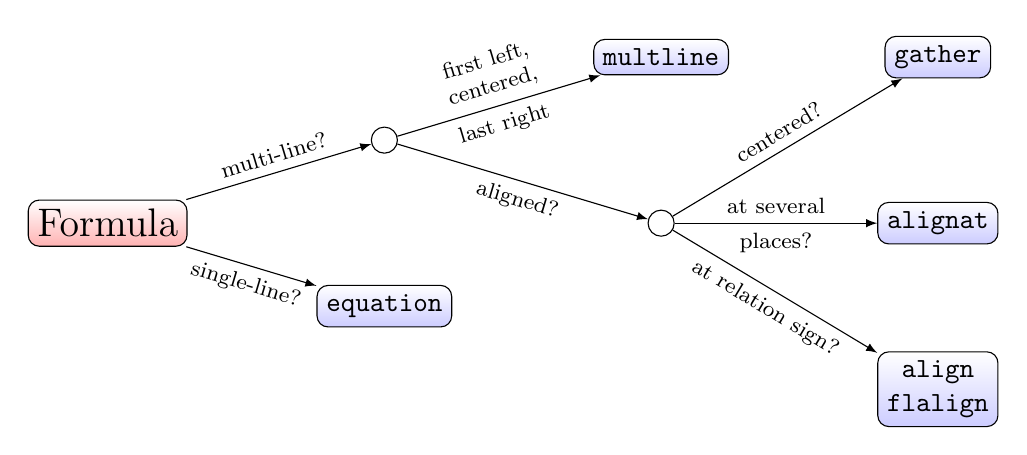
\begin{tikzpicture}
  [
    grow                    = right,
    sibling distance        = 6em,
    level distance          = 10em,
    edge from parent/.style = {draw, -latex},
    every node/.style       = {font=\footnotesize},
    sloped
  ]
  \node [root] {Formula}
    child { node [env] {equation}
      edge from parent node [below] {single-line?} }
    child { node [dummy] {}
      child { node [dummy] {}
        child { node [env] {align\\flalign}
          edge from parent node [below] {at relation sign?} }
        child { node [env] {alignat}
          edge from parent node [above] {at several}
                           node [below] {places?} }
        child { node [env] {gather}
                edge from parent node [above] {centered?} }
        edge from parent node [below] {aligned?} }
      child { node [env] {multline}
              edge from parent node [above, align=center]
                {first left,\\centered,}
              node [below] {last right}}
              edge from parent node [above] {multi-line?} };
\end{tikzpicture}
\end{document}